Spamiętanie wszystkich skrótów klawiaturowych może być trudne, zwłaszcza gdy mamy do czynienia z programami, które mają ich wiele do dyspozycji. Często też niektóre programy nie posiadają przycisków w oknie programu lub skrótów do pewnych funkcji, ukrytych gdzieś głęboko za którymś z~przycisków na pasku menu. Często jest tak, że pamiętamy nazwę funkcji, ale już nie bardzo miejsce, w którym się ona znajduje. Tu z pomocą przychodzi \textcolor{ubuntu_orange}{HUD} (Heads-up Display).

HUD jest silnie zintegrowanym narzędziem, które przy wykorzystaniu klawiatury pozwala dotrzeć nie tylko do najczęściej wykorzystywanych funkcji programu, ale również tych, o których często zapominamy, gdyż są zaszyte gdzieś głęboko. Przykładowe wykorzystanie HUD-a do skopiowania pliku:

\begin{center}
	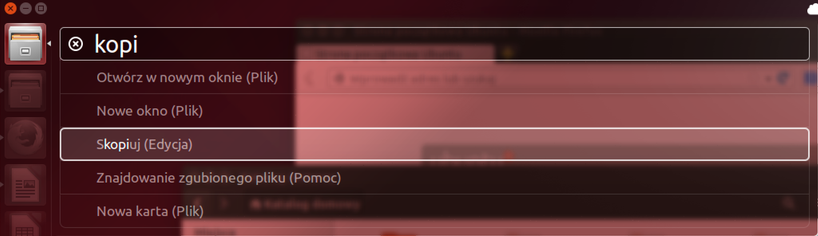
\includegraphics[width=\linewidth]{images/unity_hud1.png}
\end{center}

Inny przykład: powiedzmy, że tworzymy dokument w programie OpenOffice Writer i potrzebujemy wstawić obiekt, czy formułę. Osobie, która z programu korzysta rzadko, znalezienie tej funkcji może zająć dłuższą chwilę. Z wykorzystaniem HUD-a jest to kwestia wpisania słowa „formuła” i wybrania odpowiedniej opcji w oknie wyników wyszukiwania.
